\documentclass{beamer}

\usepackage{xcolor}
\usepackage{graphicx}
\usepackage{tcolorbox}
\usepackage{listings}
\usepackage{tabularx}
\usepackage{float}

\usetheme{metropolis}

\begin{document}

\title{Competitive Programming}
\subtitle{An introduction to the art...}
\author{University of Engineering and Technology UTEC}

\maketitle

\section{Introduction}

\begin{frame}
	\frametitle{What is Competitive Programming?}

	\begin{itemize}
		\item It's a sport... a \textbf{\textit{mind sport}}.
		\item It's simple: Participants are given problems and they have to create computer programs to solve them.
		\item The most important part is the \textbf{idea} behind the solution, not the program itself.
		\item There are many \textit{paradigms} to solve problems, we will learn more about these later...
	\end{itemize}
\end{frame}

\begin{frame}
	\frametitle{What is the ICPC?}

	\begin{itemize}
		\item \textbf{I}nterntational \textbf{C}ollegiate \textbf{P}rogramming \textbf{C}ontest
		\item Thousands of students from around the globe participate every year and attempt to became \#1 in the world.
		\item Two rounds: Regionals $\rightarrow$ World Finals
	\end{itemize}

	\begin{minipage}{0.25\linewidth}
		
\includegraphics[width=1\linewidth]{images/ICPC}
	\end{minipage}
	\hfill
	\begin{minipage}{0.7\linewidth}
		\textit{``Quite simply, it is the oldest, largest, and most prestigious programming contest in the world.''}
		\begin{flushright}
			- ICPC Webpage
		\end{flushright}
	\end{minipage}
\end{frame}

\begin{frame}
	\frametitle{Other Competitions}

	\begin{itemize}
		\item Google's Code Jam
		\item Facebook Hacker Cup
		\item IEEEXtreme
		\item TopCoder Open
	\end{itemize}

	\begin{centering}
		\setlength\tabcolsep{15pt}.
		\begin{tabular}{ c c }
			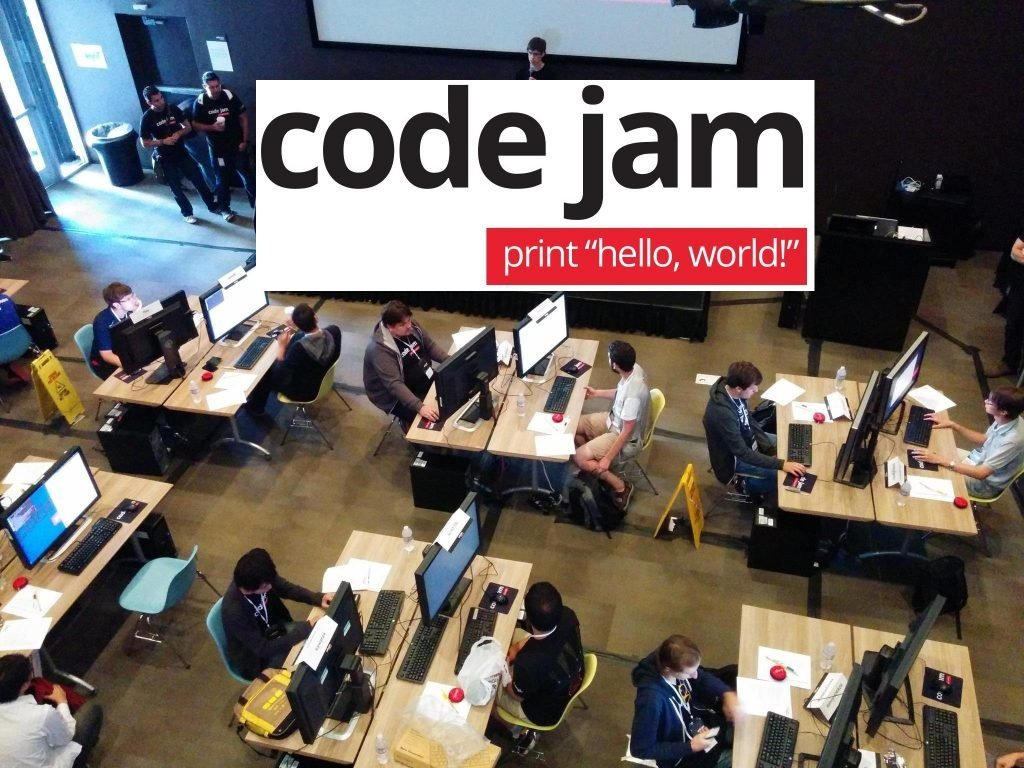
\includegraphics[width=0.4\linewidth]{images/CodeJam} &
			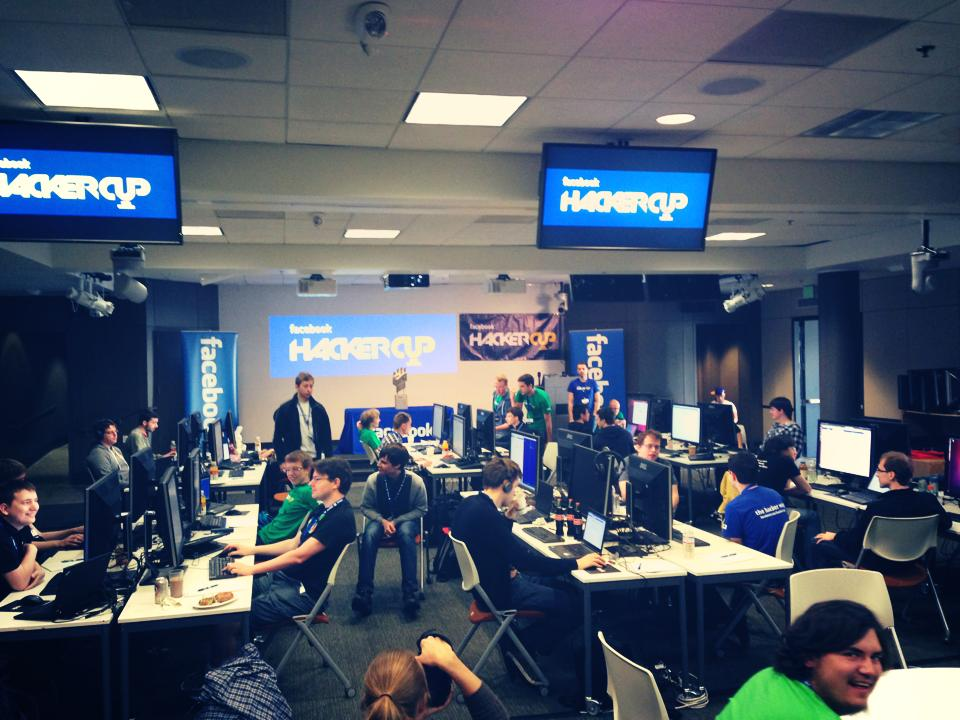
\includegraphics[width=0.4\linewidth]{images/hackercup}
		\end{tabular}
	\end{centering}
\end{frame}

\begin{frame}
	\frametitle{Virtual Judges}

	\begin{itemize}
		\item It is impossible that a human checks all of the users submissions.
		\item Virtual Judges (VJ) are the ones in charged of validating the correctness of your solution.
		\item They will run a lot of test cases with your code to make sure it \textbf{ALWAYS} work.
	\end{itemize}
\end{frame}

\begin{frame}
	\frametitle{Useful Platforms}

	\begin{itemize}
		\item Codeforces - \url{https://codeforces.com}
		\item Codechef - \url{https://www.codechef.com}
		\item AtCoder - \url{https://atcoder.jp}
		\item HackerRank - \url{https://www.hackerrank.com}
		\item UVA - \url{https://uva.onlinejudge.org}
		\item Vjudge - \url{https://vjudge.net}
	\end{itemize}
\end{frame}

\begin{frame}
	\frametitle{Problem Structure}

	\begin{itemize}
		\item Title and limitations
		\item Description
		\item Input and output (I/O)
		\item Examples
	\end{itemize}

	\textbf{Lets see the real thing:}
	\url{https://codeforces.com/contest/1/problem/A}
\end{frame}

\begin{frame}
	\frametitle{Programming Languages}

	\begin{itemize}
		\item They are the tool that allow us to give instructions to the machine.
		\item Every programming language has a purpose.
		\item In competitive programming some languages are \textit{objectively} better than others.
		\item Not all PLs are allowed in the \textit{ACM-ICPC} or other competitions.
	\end{itemize}
\end{frame}

\begin{frame}
	\frametitle{Common Programming Languages}

	\vspace{2mm}
	\begin{centering}
		\bgroup
		\def\arraystretch{5}
		\setlength\tabcolsep{35pt}.
		\begin{tabular}{ c c }
			
\includegraphics[width=0.23\linewidth]{images/java} &
			
\includegraphics[width=0.25\linewidth]{images/kotlin} \\
			
\includegraphics[width=0.25\linewidth]{images/python} &
			
\includegraphics[width=0.25\linewidth]{images/cpp}
		\end{tabular}
		\egroup
	\end{centering}
\end{frame}

\begin{frame}
	\frametitle{Why C++ is the Best}

	\begin{itemize}
		\item Lower Level $\rightarrow$ More control
		\item Allows for better memory management.
		\item It has the \textbf{STL Library}, an extremely powerful tool.
		\item Almost all learning resources are oriented to C++.
	\end{itemize}
\end{frame}

\definecolor{darkGreen}{RGB}{56,118,29}
\begin{frame}
	\frametitle{Errors - Verdict Information}

	\begin{itemize}
		\item \textcolor{darkGreen}{\textbf{AC - Accepted}}
		\item \textcolor{red}{\textbf{WA - Wrong Answer}}
		\item \textcolor{red}{\textbf{TLE - Time Limit Exceeded}}
		\item \textcolor{red}{\textbf{RE - Runtime Error}}
	\end{itemize}

	Others: \url{https://icpcarchive.ecs.baylor.edu/index.php?option=com_content&task=view&id=14&Itemid=30}
\end{frame}

\begin{frame}
	\frametitle{Setups \& IDEs}

	\begin{itemize}
		\item There are 3 main setups:
		\begin{itemize}
			\item IDE
			\item Text Editor
			\item Console Text Editor
		\end{itemize}
		\item What are some advantages and disadvantages of these?
		\item Which one should I use?
	\end{itemize}

	\vspace{5mm}

	\begin{centering}
		\setlength\tabcolsep{25pt}.
		\begin{tabular}{ c c c }
			
\includegraphics[width=0.15\linewidth]{images/clion} &
			
\includegraphics[width=0.15\linewidth]{images/sublime} &
			
\includegraphics[width=0.15\linewidth]{images/vim}
		\end{tabular}
	\end{centering}

\end{frame}

\begin{frame}
	\frametitle{Topics we will cover}

	\begin{itemize}
		\item Introduction to Programming
		\item Asymptotic Analysis
		\item Brute Force
		\item Divide and Conquer
		\item Graphs (Hopefully)
	\end{itemize}
\end{frame}

\begin{frame}
	\frametitle{Summing up}

	\begin{itemize}
		\item What is competitive programming?
		\item What is a Virtual Judge?
		\item Why are we learning C++?
		\item \emph{Why do \textbf{I} want to get into competitive programming?}
	\end{itemize}
\end{frame}

\section{Introduction to Programming}

\begin{frame}
	\frametitle{The Basics}

	\textbf{Objective:} To form a basic understanding of what is a computer program and being able to make a simple one.

	\textbf{Introductory Questions:}
	\begin{itemize}
		\item What can a computer do?
		\item How does a computer solves problems?
		\item What is an algorithm?
	\end{itemize}
\end{frame}

\begin{frame}
	\frametitle{What is a Program?}

	\begin{itemize}
		\item It a sequence of instructions the computer will execute.
		\item Programs are composed of \textit{variables and instructions}.
		\item In practice we write programs as files that we then \textit{compile} to make an \textit{executable}.
	\end{itemize}

	\begin{center}
		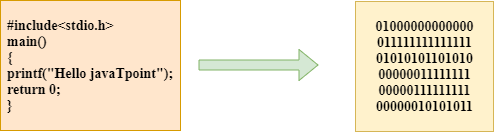
\includegraphics[scale=0.5]{images/program}
	\end{center}
\end{frame}

\begin{frame}
	\frametitle{Variables}

	\begin{itemize}
		\item A variable is a value that can change.
		\item Variables need to be \textit{declared}.
		\item It has a \textit{unique name} so that the program can identify it.
		\item Variables are stored in \textit{memory}, with a \textit{fixed} size.
		\item There are different types of variables or \textit{data types}.
		\item In \texttt{C++} we need to specify the data type of our variables.
	\end{itemize}
\end{frame}

\begin{frame}
	\frametitle{Data Types in C++}

	\begin{table}[]
		\bgroup
		\def\arraystretch{1.5}
		\setlength\tabcolsep{10pt}.
		\begin{tabular}{l|l|l}
			\multicolumn{1}{c|}{\textbf{Type}} & \multicolumn{1}{c|}{\textbf{Size}} & \multicolumn{1}{c}{\textbf{Range}} \\ \hline
			\texttt{short} & 16 bit & $[-2^{15}, 2^{15} - 1]$ \\
			\texttt{int} & 32 bit & $[-2^{31}, 2^{31} - 1]$ \\
			\texttt{long long} & 64 bit & $[-2^{63}, 2^{63} - 1]$ \\
			\texttt{float} & 32 bit & $[-3.4 \times 10^{38}, 3.4 \times 10^{38} - 1]$ \\
			\texttt{double} & 64 bit & $[-1.7 \times 10^{308}, 1.7 \times 10^{308}]$ \\
			\texttt{char} & 8 bit & $[-2^{7}, 2^{7} - 1]$						  
		\end{tabular}
		\egroup
	\end{table}
\end{frame}
	
\begin{frame}
	\frametitle{Arithmetic Operators}

	\begin{itemize}
		\item The name pretty much gives everything away.
		\item We need to be careful with data types.
		\item Operators obey the laws of order of operator.
	\end{itemize}

	\begin{tcolorbox}[title=Operators]
		\begin{itemize}
			\item[--] \texttt{10 + 5} $\rightarrow 15$
			\item[--] \texttt{10 - 5} $\rightarrow 5$
			\item[--] \texttt{10 * 5} $\rightarrow 50$
			\item[--] \texttt{10 / 5} $\rightarrow 2$
			\item[--] \texttt{10 \% 5} $\rightarrow 0$
		\end{itemize}
	\end{tcolorbox}
\end{frame}

\lstset{
	basicstyle=\footnotesize\ttfamily,
	tabsize=4, % tab space width
	showstringspaces=false, % don't mark spaces in strings
	commentstyle=\color{grey}, % comment color
	keywordstyle=\color{blue}, % keyword color
	stringstyle=\color{purple} % string color
}

\begin{frame}[fragile]
	\frametitle{Lets see the real thing - \texttt{Hello World}}

	\begin{lstlisting}[language=C++]
#include <iostream>
using namespace std;

int main() {
	cout << "Hello World!" << endl;
	return 0;
}
	\end{lstlisting}
\end{frame}

\begin{frame}[fragile]
	\frametitle{Flow Control - if, else}

	\begin{lstlisting}[language=C++]
int main() {
	int x;
	cin >> x;
	if (x < 0) {
		cout << x << " is smaller that 0!" << endl;
	}
	else {
		cout << x << " is greater than 0!" << endl;
	}
	return 0;
}
	\end{lstlisting}
\end{frame}

\begin{frame}[fragile]
	\frametitle{Flow Control - else if}

	\begin{lstlisting}[language=C++]
int main() {
	int x;
	cin >> x;
	if (x < 0) {
		cout << x << " is smaller that 0!" << endl;
	}
	else if (x == 0) {
		cout <<x << " is equal to 0!" << endl;
	}
	else{
		cout << x << " is greater than 0!" <<endl;
	}
	return 0;
}
	\end{lstlisting}
\end{frame}

\begin{frame}[fragile]
	\frametitle{Loops - while}

	\begin{lstlisting}[language=C++]
int main(){
	int i = 0;
	while (i < 5) {
		cout << i << ' ';
	}
	cout << endl;
	return 0;
}
	\end{lstlisting}
\end{frame}

\begin{frame}[fragile]
	\frametitle{Loops - for}

	\begin{lstlisting}[language=C++]
int main() {
	for (int i = 0; i < 5; i++) {
		cout << i << ' ';
	}
	cout << endl;
	return 0;
}
	\end{lstlisting}
\end{frame}

\begin{frame}[fragile]
	\frametitle{Functions}

	\begin{lstlisting}[language=C++]
int square(int n) {
	int answer = n * n;
	return answer;
}

int main() {
	cout <<square(5) << endl;
	cout << square(7) << endl;
	return 0;
}
	\end{lstlisting}
\end{frame}

\begin{frame}[fragile]
	\frametitle{Functions}

	\begin{lstlisting}[language=C++]
int main() { 
	int arr0[5];
	int arr1[4] = {1,2,3,4};
	int arr2[5] = {1,2,3,4};
 
	cout << arr0[0] << endl;
	cout << arr1[1] << endl;
	cout << arr2[4] << endl;
	cout << arr2[5] << endl;
	cout << arr1[5] << endl;
	return 0;  
}
	\end{lstlisting}
\end{frame}

\section{Problem Time}

\begin{frame}
	\frametitle{Problem - Description}

	\textbf{Time Limit:} 1s \\
	\textbf{Memory Limit:} 256MB

	There are $n$ flowers in a park numbered from $1$ to $n$. Each flower has a number that defines its beauty, in general the $i$th flower has a beauty of $b_i$ for $1 \leq i \leq n$. 
	
	Leonidas is in this park flower picking. Because he loves this park so much, he has a rule of picking a maximum of 2 flowers per visit. In this occasion, he wants to pick the pair of flowers such that the sum of their beauties is maximum. Leonidas doesn't know which flowers to pick, can you help him out?
\end{frame}

\begin{frame}
	\frametitle{Problem - I/O}

	\textbf{Input:}

	The first line contains $n$ ($1 \leq n \leq 10^6$), the number of flowers in the park. The next line contains $n$ integers, representing $b_1$, $b_2$, $b_3$, ... $b_n$  ($0 \leq b_i \leq 10^6$).

	\textbf{Output}

	The maximum sum of the beauty of two flowers.

\end{frame}

\begin{frame}
	\frametitle{Problem - Examples}

	\textbf{Example 1:}
	\vspace{2mm}
	\begin{columns}
		\begin{column}{0.3\textwidth}
			\begin{tcolorbox}[fonttitle=\bfseries, title=Input]
				5\\
				12 23 45 25 8
			\end{tcolorbox}
		\end{column}
		\begin{column}{0.3\textwidth}
			\begin{tcolorbox}[fonttitle=\bfseries, title=Output]
				70\\
			\end{tcolorbox}
		\end{column}
	\end{columns}

	\vspace{4mm}

	\textbf{Example 2:}
	\vspace{2mm}
	\begin{columns}
		\begin{column}{0.3\textwidth}
			\begin{tcolorbox}[fonttitle=\bfseries, title=Input]
				4\\
				1 1 1 1
			\end{tcolorbox}
		\end{column}
		\begin{column}{0.3\textwidth}
			\begin{tcolorbox}[fonttitle=\bfseries, title=Output]
				2\\
			\end{tcolorbox}
		\end{column}
	\end{columns}
\end{frame}

\end{document}
